\chapter{Experimental Apparatus}


\section{Particle Accelerators}

	To study the Standard Model, the Higgs boson, and hints of new physics, particle accelerators are used. Particle accelerators can be categorized as either fixed target or colliders. As the naming suggest, in a fixed target accelerator the beam hits a target that then produces the desired particle collisions. Whereas a collider uses two opposite circulating beams that are then brought to collide inside a detector. A fixed target accelerator energy scales as $E_{CM} = \sqrt{E_{beam}}$ whereas a collider scales as $E_{CM} = 2 \, E_{beam}$. 

	\subsection{Hadron Colliders}

		There are two main types of particle colliders, those that use hadrons and those that use leptons. Lepton colliders are often referred to as precision machines, as the longitude momentum is known and backgrounds are well understood. The center of mass energy is well controlled in a lepton collider, meaning particles can be produced on resonance. On the other hand, due to the nature of hadrons not being fundamental particles a hadron collider produces a wide range of collisions. The constituents of a hadron participate in the collisions, meaning it is impossible to know the exact longitude momentum of the initial state. It is because of this exact reason that hadron colliders are referred to as discovery machines. The synchrotron radiation produced from a hadron collider is much lower than that of a lepton collider; meaning the beams are easier to control and can be pushed to higher energies without extra loses. The center of mass energy scales with $\frac{1}{m^4}$ in a hadron collider; again leading to an increased energy gain by simply using heavier particles.

	\subsection{The Large Hadron Collider}

		The Large Hadron Collider (LHC) is a 27 km circumference circular collider built outside of Geneva, Switzerland at CERN (Conseil Européen pour la Recherche Nucléaire). At center of mass energy $13.6$ TeV, the LHC is the largest and highest energy particle accelerator ever built. There are four main collision points along the LHC: the ATLAS, CMS, ALICE, and LHCb experiments. ATLAS and CMS are general purpose particle detectors while ALICE and LHCb focus on heavy ion collisions. The numbers stated in the following sections are in reference to proton-proton collisions.

		The LHC consists of 1104 NbTi superconducting dipole magnets, each being 15 m long, weighing 35 tonnes, cooled to 2 K, operating at 11,000 Amps, and produce a magnetic field of 8.3 T. A cross-section of a dipole magnet and the surrounding cryogenic system can be see in figure \ref{fig:dipole-xsec}. The dipole magnets are used to bend the beam around the ring with another 128 used in the beam dump system to remove the beam safely from the LHC. A 2-in-1 configuration is used within the dipole magnets to create the required magnetic fields to bend two equally charged beams in opposite directions. A diagram of the magnetic fields in this configuration produced can be seen in \ref{fig:dipole-field}. To focus the beam in the horizontal and vertical planes two quadrapole magnets are used; one magnet focuses in one plane while defocusing in the other. The end result is a horizontally and vertically focused beam. While in the LHC, the hadrons are accelerated using radiofrequency cavities. Table \ref{tab:LHC} lists some information on the LHC. 

		\begin{table}[!thp]
			\centering
			\caption{LHC parameters  ~\cite{lhc-facts}}
			\begin{tabular}{| l | l |}  
			\hline
			Circumference 						& $26,659$ m 					\\ 	\hline
			Dipole operating temperature 		& $1.9$ K 						\\ 	\hline
			Dipole magnets 						& $1232$ 						\\	\hline
			Quadrapole magnets 					& $392$ 						\\	\hline
			Radiofrequency cavities 			& $16$ ($8$ per beam) 			\\ 	\hline
			Beam energy 						& $6.5$ TeV ($13$ CoM TeV) 		\\ \hline
			Protons per bunch 					& $1.2 \mathrm{x} 10^11$ 		\\ \hline
			Bunches per beam 					& $2808$ 						\\ \hline
			Revolutions per second 				& $11245$ 						\\ \hline
			Collisions per second 				& $1,000,000,000$ 				\\ \hline
			\end{tabular}
			\label{tab:LHC}
		\end{table}

		\begin{figure}[!ht]
		\centering
		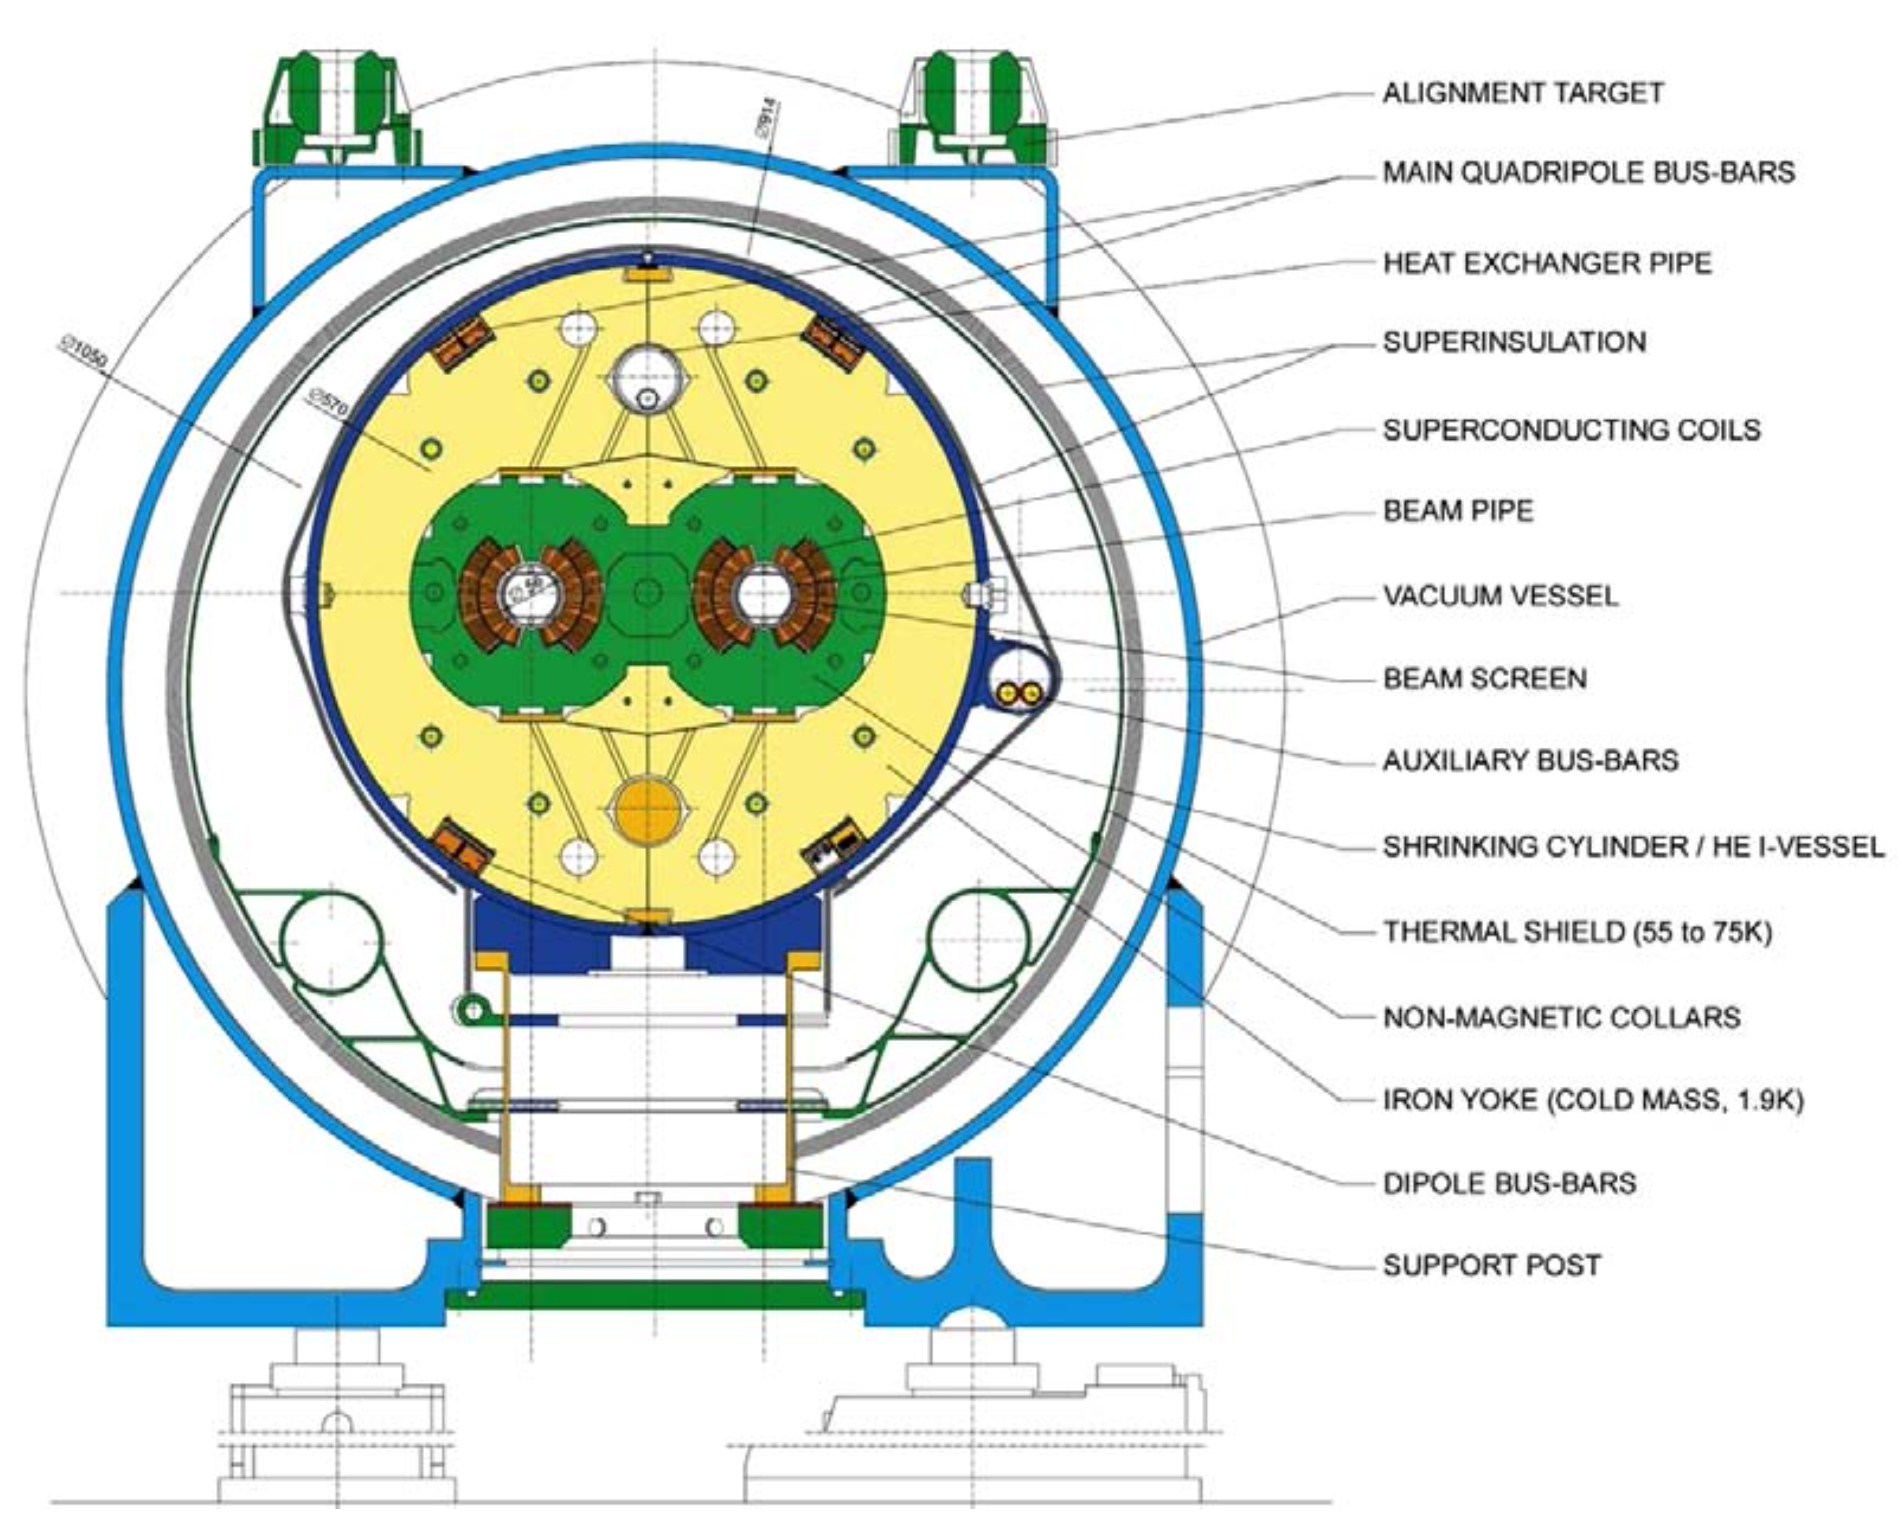
\includegraphics[width=\textwidth,keepaspectratio=true]{chapters/chapter2_experiment/images/dipole-crosssection.png}
		\caption{Cross-section of cryodipole (lengths in mm). \cite{lhc-machine}}
		\label{fig:dipole-xsec}
		\end{figure}

		\begin{figure}[!ht]
		\centering
		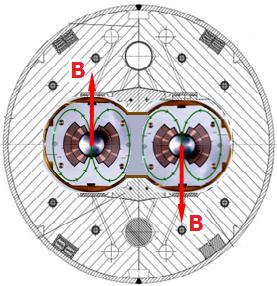
\includegraphics[width=.45\textwidth,keepaspectratio=true]{chapters/chapter2_experiment/images/dipole-field.jpeg}
		\caption{Field of the LHC dipole magnets. \cite{dipole-field}}
		\label{fig:dipole-field}
		\end{figure}

	\subsection{CERN Accelerator Complex}
		There are a series of accelerators used to get each beam up to its final energy of 6.5 TeV. The protons used in collisions are sourced from hydrogen atoms. The hydrogen is ionized, leaving the nucleus consisting of one proton, these protons are then accelerated in radiofrequency (RF) cavities. Figure \ref{fig:CERN-complex} shows in detail the full accelerator complex at CERN. 
		\begin{figure}[!ht]
		\centering
		\includegraphics[width=\textwidth,keepaspectratio=true]{chapters/chapter2_experiment/images/CERN-complex.png}
		\caption{The CERN accelerator complex. \cite{CERN-complex}}
		\label{fig:CERN-complex}
		\end{figure}
		The protons used in the LHC start the accelerating process in the linear accelerator LINAC 2. They then are accelerated in the booster, PS, SPS, and are finally injected at the LHC where they are accelerated to the final 6.5 TeV beam energy. The final energies of protons from each accelerator can be seen in Table \ref{tab:accelerator-complex}.
		\begin{table}[!thp]
			\centering
			\caption{Accelerator final energies}
			\begin{tabular}{| l | l |}  
			\hline
			Accelerator 					& Final Energy 	\\ \hline
			\hline
			LINAC 2 						& $50$ MeV 		\\ 	\hline
			Booster 						& $1.4$ GeV 	\\ 	\hline
			Proton Synchrotron (PS)			& $26$ GeV 		\\ 	\hline
			Super Proton Synchrotron (SPS) 	& $450$ GeV 	\\ 	\hline
			Large Hadron Collider (LHC)		& $6.5$ TeV 	\\ 	\hline
			\end{tabular}
			\label{tab:accelerator-complex}
		\end{table}

	\subsection{Luminosity}
		The amount of data collected from colliders is often referred to in terms of luminosity. Luminosity is measured in terms of inverse barns, where $1 \, b = 10^{-28} \, m^2$. Instantaneous luminosity of one bunch crossing can be written as 
		\begin{equation}\label{eqn:bunch-lumi}
		\mathcal{L}_{bunch} = \frac{ \mu  f }{\sigma}
		\end{equation}
		where $\sigma$ is the cross section and can be thought of as the probability of a collision occurring, $\mu$ is the number of inelastic interactions per bunch crossing, and $f$ is the revolution frequency of the LHC $f=11246$ Hz. Therefore, the total instantaneous luminosity is 
		\begin{equation}\label{eqn:tot-inst-lumi}
		\mathcal{L} = N_b \frac{ \langle \mu \rangle f}{\sigma}
		\end{equation}
		where $\langle \mu \rangle$ is the average number of inelastic interactions per bunch crossing. 

		The integrated luminosity then corresponds to the total amount of data that was taken during a time period and can be seen for the LHC Run-2 in \ref{fig:lhc-lumi}
		\begin{figure}[!ht]
		\centering
		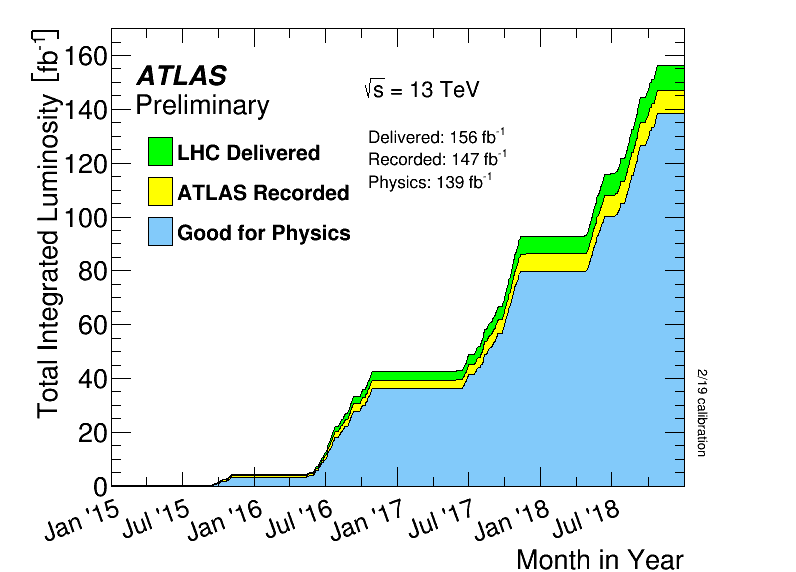
\includegraphics[width=.65\textwidth,keepaspectratio=true]{chapters/chapter2_experiment/images/intlumivstimeRun2DQall.png}
		\caption{ Cumulative luminosity versus time delivered to ATLAS (green), recorded by ATLAS (yellow), and certified to be good quality data (blue) during stable beams for pp collisions at 13 TeV center of mass energy in 2015-2018. The difference between the colored histograms reflects inefficiencies, especially those seen when restarting data taking. }
		\label{fig:lhc-lumi}
		\end{figure}
		The value of $\langle \mu \rangle$ changed throughout data taking and can be seen in Figure \ref{fig:run2-mu} and is referred to as pileup because the higher the $\langle \mu \rangle$ value, the more messy a collision becomes.
		\begin{figure}[!ht]
		\centering
		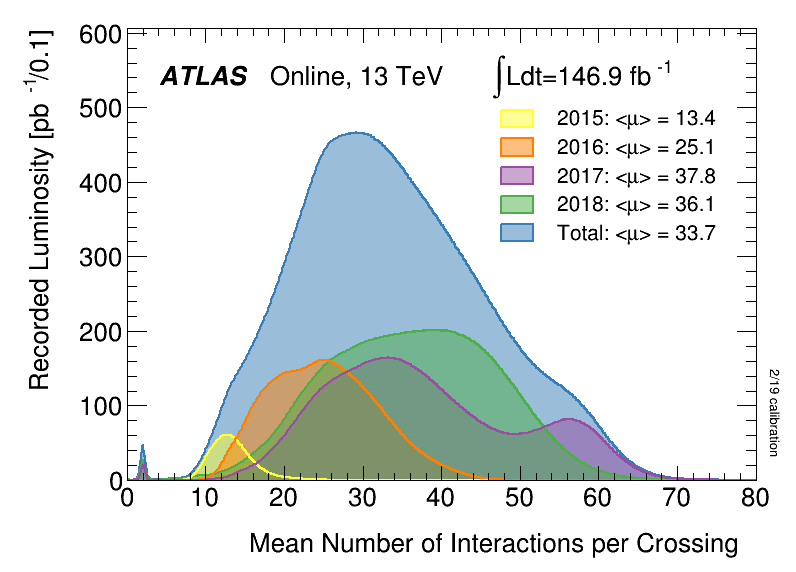
\includegraphics[width=.65\textwidth,keepaspectratio=true]{chapters/chapter2_experiment/images/mu_2015_2018.png}
		\caption{ The luminosity-weighted distribution of the mean number of interactions per bunch crossing for the 2015-2018 \pp collision dataset at $13$ TeV center of mass energy. }
		\label{fig:run2-mu}
		\end{figure}

		A common calculation using the total integrated luminosity is shown in Equation \ref{eqn:tot-proc-num}; where the number of times a particular process was produced is calculated.
		\begin{equation}\label{eqn:tot-proc-num}
		N_{x} = \mathcal{L} \sigma_{x}
		\end{equation}
		where again, $\sigma$ is the cross section. In this case, the cross section corresponding to process $x$.


\section{The ATLAS Detector}
	The ATLAS (\textbf{A} \textbf{T}oroidal LHC \textbf{A}pparatu\textbf{S}) detector is one of two general purpose particle detectors on the LHC. The other being the \textbf{C}ompact \textbf{M}uon \textbf{S}olenoid (CMS). ATLAS, like other particle detectors, is comprised of four main components; the inner detector, calorimeters, muon system, and the magnet system. Each component has several types of technology in order to measure the energy of all possible particle decays.\footnote{Neutrinos are not directly detected, but inferred via a missing transverse energy calculation described in Section \ref{sec:etmiss}.} Figure \ref{fig:ATLAS} shows a 3D model of the ATLAS detector.

	\begin{figure}[!ht]
	\centering
	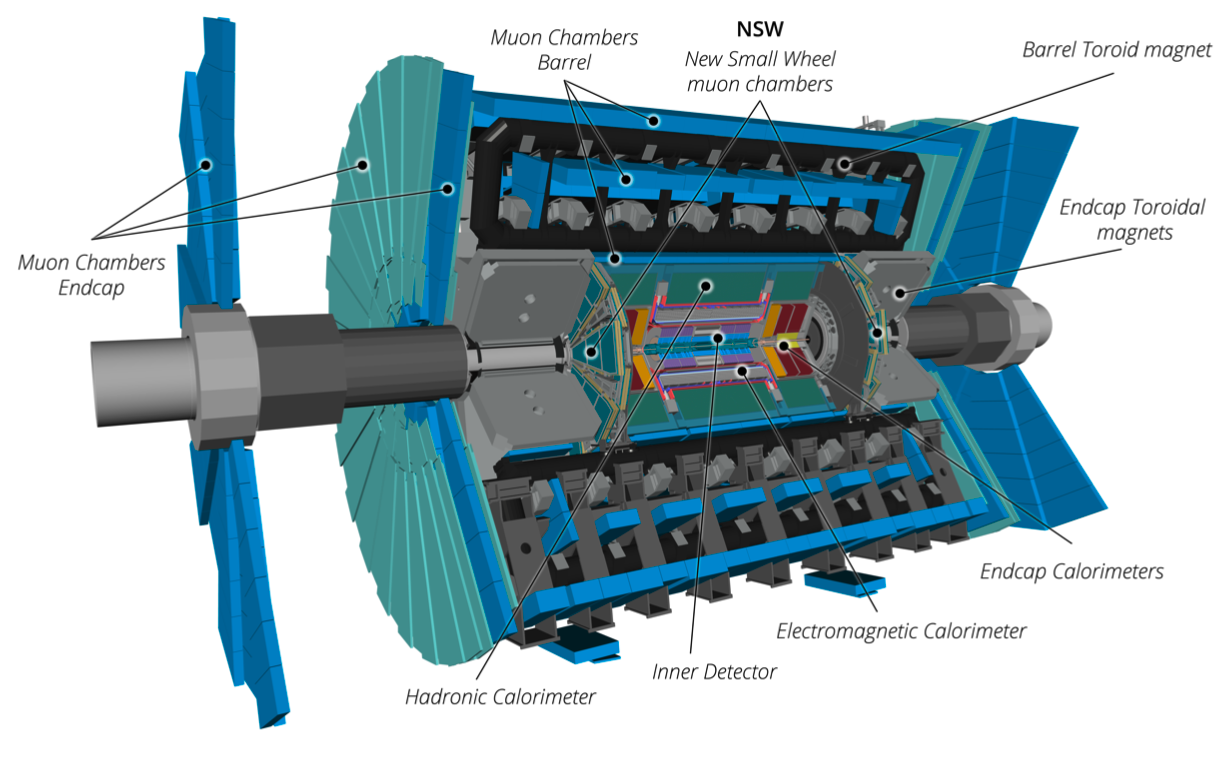
\includegraphics[width=\textwidth,keepaspectratio=true]{chapters/chapter2_experiment/images/ATLAS_3d_run3.png}
	\caption{ The ATLAS detector with major subdetectors highlighted.}
	\label{fig:ATLAS}
	\end{figure}

	\subsection{Detector Coordinates}
	Since ATLAS is a cylinder, it is convenient to start with polar cylindrical coordinates. For ATLAS, the z-axis is inline with the beam line, the x-axis points towards the center of the LHC ring, and the y-axis points vertically. However, since particle collisions are relativistic by nature, a set of Lorentz invariant coordinates is much more useful. The radial coordinate r defines the radial distance from the interaction point (IP) at the center of ATLAS, $\phi$ is the azimuthal angle describing the angle from the x-axis in, and $\eta$, the pseudorapidity, is defined as 
	\begin{equation}\label{eqn:eta}
	\eta \equiv - ln(tan(\frac{\theta}{2}))
	\end{equation}
	where $\theta$ is the angle from the y-axis. It is in the differences in $\eta$ between particles that provides the Lorentz invariance in this coordinate system of $(r,\phi,\eta)$. Due to the large collision energies of the LHC, the pseudorapidity is a close estimate to the true rapidity of the particles. 
	\begin{equation}\label{eqn:rapidity}
	y \equiv \frac{1}{2} ln(\frac{E+p_Z}{E-p_Z}) \approx \eta
	\end{equation}
	When speaking of differences in particle locations within ATLAS, $\Delta R$  is often used.
	\begin{equation}\label{eqn:dR}
	\Delta R \equiv \sqrt{ (\Delta \eta)^2 + (\Delta \phi)^2}
	\end{equation}

	\subsection{Inner Detector}

		\subsubsection{Pixel}

		\subsubsection{Semiconductor Tracker}

		\subsubsection{Transition Radiation Tracker}

	\subsection{Calorimeters}

		\subsubsection{Liquid Argon Electromagnetic Calorimeter}

		\subsubsection{Tile Hadronic Calorimeter}

	\subsection{Muon System}

		\subsubsection{Monitored Drift Tubes}

		\subsubsection{Cathode Strip Chambers}

		\subsubsection{Resistive Plate Chambers} 

		\subsubsection{Thin Gap Chambers}

	\subsection{Magnet Systems}

		\subsubsection{Solenoid Magnet}

		\subsubsection{Toroid Magnet}

		